\section{Présentation} % (fold)
\label{sub:pr_sentation}
	Pour ce premier programme, la technique de segmentation utilisée a été la binarisation par seuillage. En regardant les images IRM, on constate en effet que la tumeur correspond à une zone plus claire. On va donc séparer l'histogramme en deux parties :\\
	\begin{itemize}

		\item les intensités les plus élevées, correspondant à la tumeur et aux autres zones de l'image ayant les mêmes niveaux de gris;
		\item les intensités les plus faibles, correspondant au reste de l'image, plus sombre.
	\end{itemize}
	\bigskip

	On constate qu'avec la binarisation, on a séparé les zones plus claires mais ces zones ne correspondent pas toutes à la tumeur. Il faut donc sélectionner la bonne zone en calculant les aires de chacun de ces régions et en affectant celle ayant la plus grande aire à la tumeur.\\

	On remarquera que cette technique comporte un hyper-paramètre, qui est le seuil de la binarisation.

% section pr_sentation (end)

\section{Résultats}
	\subsection{Binarisation} % (fold)
	\label{ssub:binarisation}
		On applique tout d'abord la binarisation, avec un seuil de 36 \%, correspondant à un niveau de gris de 91. On visualise l'histogramme avant (figure \ref{fig:hist}) et après la binarisation (figure \ref{fig:histBinaire}). On peut le faire pour chaque IRM segmentée. Les images présentées ici correspondent à l'image avant traitement.

		\begin{figure}[H]
			\centering
			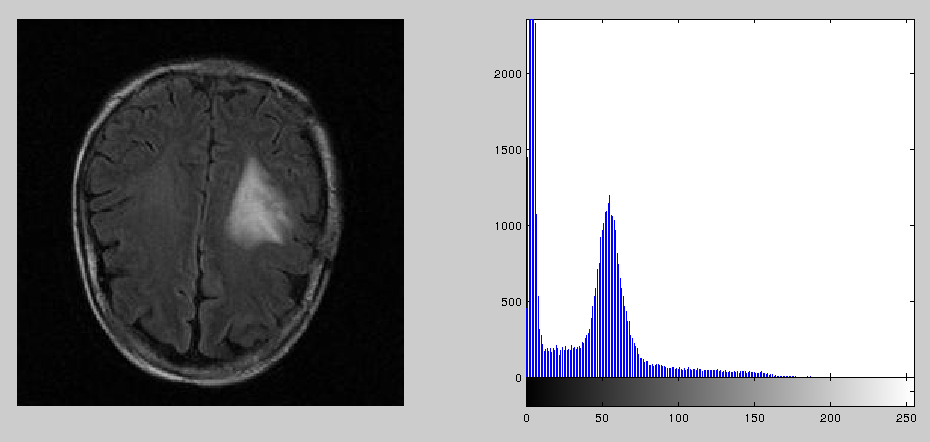
\includegraphics[width=\textwidth]{images/1-hist.png}
			\caption{Image et histogramme avant la binarisation}
			\label{fig:hist}
		\end{figure}

		\begin{figure}[H]
			\centering
			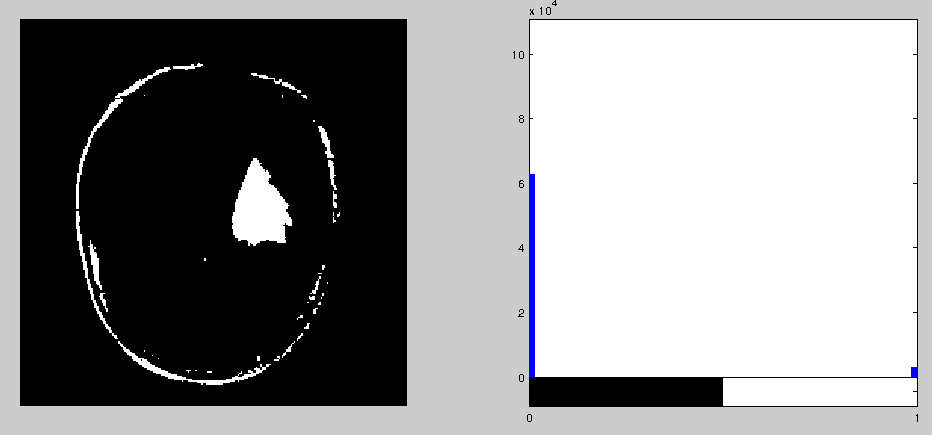
\includegraphics[width=\textwidth]{images/1-histBinaire.png}
			\caption{Image et histogramme après la binarisation}
			\label{fig:histBinaire}
		\end{figure}

		On constate qu'il y a plusieurs zones blanches sur l'image binarisée. On cherche à ne conserver que celle correspondant à la tumeur.
	% subsection binarisation (end)

	\subsection{Conservation de la plus grande zone blanche} % (fold)
	\label{ssub:conservation_de_la_plus_grande_zone_blanche}
		Pour conserver uniquement la tumeur parmi les zones plus claires identifiées, on calcule l'aire de chaque zone. On dit ensuite que la tumeur est la zone ayant l'aire la plus importante. Les résultats obtenus sont présentés dans la figure \ref{fig:tumeurBinaire}.

		\begin{figure}[H]
			\centering
			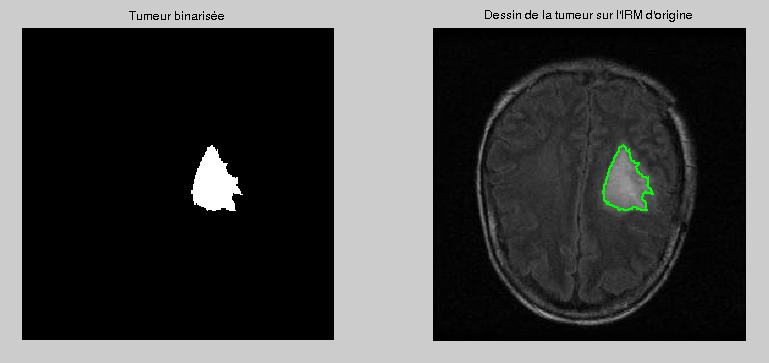
\includegraphics[width=\textwidth]{images/1-tumeur.png}
			\caption{Segmentation de la tumeur sur l'IRM avant traitement}
			\label{fig:tumeurBinaire}
		\end{figure}

	% subsection conservation_de_la_plus_grande_zone_blanche (end)

	\subsection{Pourcentage d'augmentation de la surface} % (fold)
	\label{ssub:pourcentage_d_augmentation_de_la_surface}
		On applique cette technique sur l'IRM avant traitement et sur l'IRM après traitement, afin d'obtenir la surface de la tumeur sur ces deux images. On calcule ensuite le changement de surface de la tumeur après le traitement. Avec cette méthode on obtient une augmentation de 6.5 \%. Cela signifie que le traitement n'a pas été efficace et que la tumeur a grandi.\\

		On ne sait cependant pas si ce résultat est bon ou si notre méthode a été peu efficace. On ne sait notamment pas à quel point un petit changement de seuil peut influencer ce résultat.
	% subsection pourcentage_d_augmentation_de_la_surface (end)

\section{Influence du seuil}
	Afin de valider le résultat obtenu précédemment, on fait varier le seuil dans des limites acceptables (de 0.35 à 0.45) afin de voir si le résultat change beaucoup. Pour chacun de ces seuils on applique la méthode de segmentation par binarisation, on calcule l'aire des tumeurs avant et après traitement et on calcule le ratio correspondant à l’augmentation de la taille de la tumeur. On visualise ces ratios dans la figure \ref{fig:ratios_binarisation}.

	\begin{figure}[H]
		\centering
		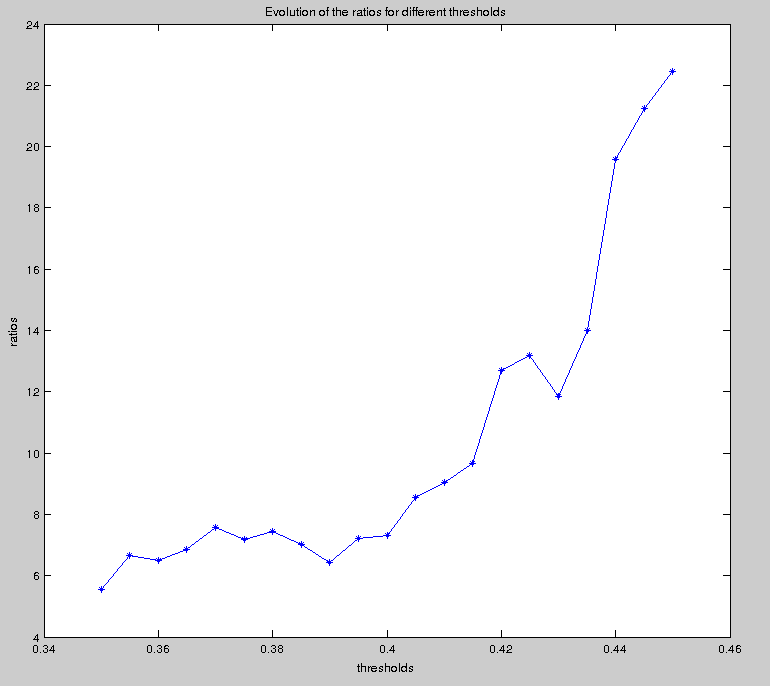
\includegraphics[width=0.75\textwidth]{images/1-ratios.png}
		\caption{Évolution du ratio d'augmentation de la taille de la tumeur pour différents seuils}
		\label{fig:ratios_binarisation}
	\end{figure}

	On voit que le ratio évolue beaucoup lorsque le seuil varie, ce qui nous amène à penser que cette méthode n'est pas stable et que notre résultat est donc peu fiable.
